% ================================= chapter 4 ================================= %
\chapter{シミュレーション}
目標値変更、振り上げ制御のシミュレーションを行い、重み行列、オブザーバの極、サンプリング周期、
パラメータ$k$, $n$を変更し、それぞれの変更による性能の違いを確かめる.

\subsection{重み行列変更に関するシミュレーション}
目標値変更における安定化制御で、表\ref{sim_Q}に示すパラメータを用いてシミュレーションを行う。

\begin{table}[htbp]
    \begin{center}
        \caption{表\ref{sim_Q}: シミュレーションに用いるパラメータの種類}
        \begin{tabular}{|c|c|c|c|c|} \hline
            パターン & 重み行列$Q$ & オブザーバの極$P$ & サンプリング周期$dt$ \\ \hline \hline
            パターン1 & (1E6, 1E5, 1, 1) & (-23, -23) & 0.005 \\ \hline
            パターン2 & (1E5, 1E6, 1, 1) & (-23, -23) & 0.005 \\ \hline
            パターン3 & (1E6, 1E6, 1, 1) & (-23, -23) & 0.005 \\ \hline
        \end{tabular}
        \label{sim_Q}
    \end{center}
\end{table}

表\ref{sim_Q}に従ってシミュレーションを行った結果を図に示す。

\begin{figure}[htbp]
    \begin{minipage}{0.5\hsize}
        \begin{center}
            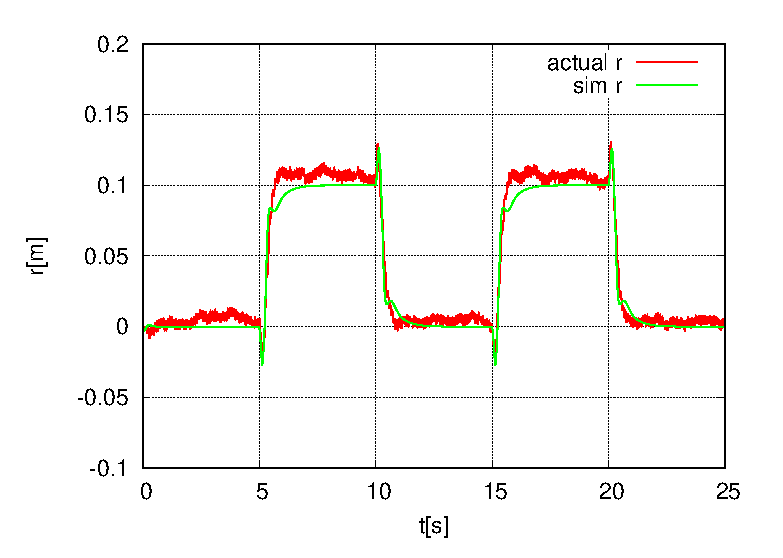
\includegraphics[width=1.0\linewidth]{case1_r.eps}
            \caption{図\ref{case01_r}: パターン1の台車位置}
            \label{case01_r}
        \end{center}
    \end{minipage}
    \begin{minipage}{0.5\hsize}
        \begin{center}
            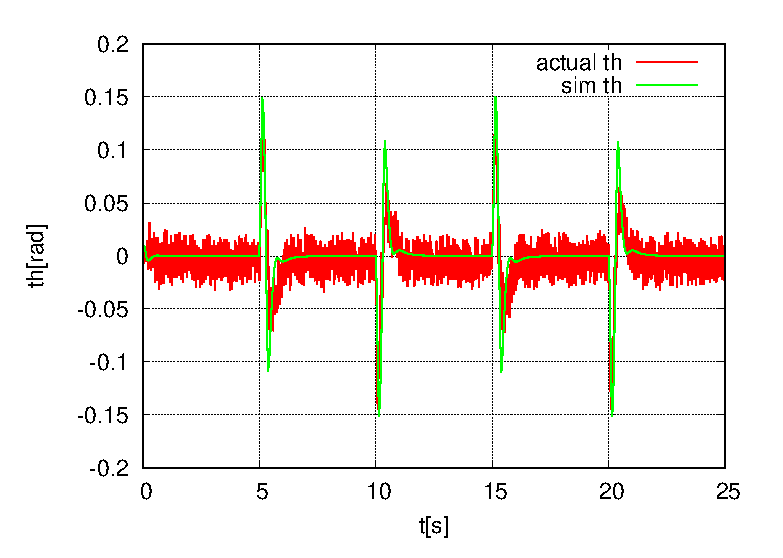
\includegraphics[width=1.0\linewidth]{case1_th.eps}
            \caption{図\ref{case01_th}: パターン1の振子角度}
            \label{case01_th}
        \end{center}
    \end{minipage}
\end{figure}

\subsection{オブザーバの極変更に関するシミュレーション}

\subsection{サンプリング周期変更に関するシミュレーション}

\subsection{振り上げ制御のシミュレーション}

\subsection{シミュレーションの考察}

% =============================== chapter 4 END =============================== %